\subsection{Computing Program Probabilities}
\label{sec:computingprobabilities}

Computing probabilities for probabilistic symbolic execution and other program analyses reduces to computing the probability of satisfying a boolean constraint over the program variables. This operation is performed within the \x{selectBranch} function. Given the path condition $PC$ reaching a branching point and the condition $c$ of the conditional statement, the goal is to compute the probability of satisfying $PC \land c$ and, consequently, $PC \land \neg c$. Depending on the theory the constraints are expressed in, different techniques can be used to quantify the solution space of the constraints and, in turn, their probability of being satisfied. In this section introduce the basics of some of these techniques.

Assume the program under analysis has input variables $V=\{v_1, v_2, \dots, v_n\}$, where $v_i$ has domain $d_i$ and comes with a probability distribution $\mathcal{P}_i: d_i \to [0, 1]$. The input domain $D$ is the Cartesian product of the domains $d_i$, while the input distribution $\mathcal{P}$ is the joint distribution over all the input variables $\prod_i \mathcal{P}_i(\bar{v_i})$. Given a constraint $\phi: V \to \{true, false\}$, the goal is to compute the probability $Pr(\phi)$ of satisfying $\phi$ given the input domains and probability distributions. 
%This problem is usually referred to as model counting, when the input domains are countable, or solution space quantification, when the input domains are modeled as uncountable (e.g., abstracting floating-point numbers as reals).

\subsubsection{Exact and numeric computation}\label{sec:computingprobabilitiesExact}

% OUTLINE
%	\begin{enumerate}
%		\item Finite domains
%			\begin{enumerate}
%				\item Linear integers (Latte, Barvinok, Omega for negation; used in our works)
%				\item Strings (bounds: \url{http://www.comp.nus.edu.sg/~shweta24/publications/smc\_pldi14.pdf} ; automata-based exact and upperbounds: \url{http://www.cs.ucsb.edu/~bultan/publications/model-counting.pdf}; we should also check the related work thereof)
%				\item Data structures (icse13 and spin15)
%				\item Sat and smt (\url{http://arxiv.org/pdf/1306.5726v3.pdf}, \url{http://arxiv.org/pdf/1411.0659.pdf}; these papers should have been published, we should check related work in there)
%			\end{enumerate}
%		
%		\item Uncountable domains
%			\begin{enumerate}
%				\item Symbolic and numerical integration (interesting, but symbolic does not scale apart from a few simple cases, while numeric suffers for large cardinality of input domains; however: general, available off-the-shelf, parallelizable for numerical)
%			\end{enumerate}
%	\end{enumerate}

\paragraph{Finite domains.} 

If the input domain is finite, the computation of $Pr(\phi)$ reduces to a counting problem as already mentioned (assume for now all inputs are uniformly distributed, i.e. they are equally likely):
%
\begin{equation}\label{eq:counting}
	Pr(\phi) = \frac{\sharp(\phi \land D)}{\sharp(D)}
\end{equation}
%
\noindent Here $\sharp(\cdot)$ counts the number of inputs satisfying the argument constraint; $D$ has been overloaded to represent the finite domain as a constraint; $\sharp(D)$ is a short form for the size of the domain\footnote{More precisely, Equation~\eqref{eq:counting} represents the probability of satisfying the constraint $\phi$ conditioned on the fact that the input is within the prescribed domain $D$.}. For example, considering a single integer input variable $x$ taking values between $1$ and $10$ uniformly, $\sharp(D)=10$ and $\sharp(x\leq5 \land D)=5$, leading to a $0.5$ probability of satisfying the constraint.

The computation of $\sharp(\cdot)$ can be performed efficiently for linear integer arithmetic (LIA) constraints.
A LIA constraint defines a multi-dimensional lattice bounded by a convex polytope~\cite{de2008computationalGeometry}. To count the number of points composing this structure, an efficient solution has been proposed by Barvinok~\cite{barvinok1994polynomial}. This algorithm uses generating functions suitable for solving the counting problem in polynomial time, with respect to the number of variables and the number of constraints. Notably, besides the number of bits required to represent the numerical values, the complexity of this algorithm does not depend on the actual size of the variable domains. This makes the computation feasible for very large input domains, allowing its application to probabilistic program analysis\cite{Geldenhuys2012,Filieri2013,Filieri2015}. Several implementations of this algorithm are available, the most popular being LattE~\cite{LattESoftware} and Barvinok~\cite{verdoolaegesoftware}. 
%When disjunctions appear in the constraint, these have to be preprocessed before applying Barvinok's algorithm (e.g., using the Omega library~\cite{Omega1996}). Though this normalization increases the overall complexity of model counting, several optimizations can mitigate the computational effort required.
%(we will discuss some later in Section~\ref{sec:computingprobabilitiesOptimizations}) 
%Barvinok's algorithm has been used for probabilistic program analysis in \cite{Geldenhuys2012,Filieri2013,Filieri2015}.


\ignore{
	\item \textbf{Bounded data structures}: data structures are usually composed of a structural dimension (e.g., lists or trees) and a payload stored in each node of the structure. The level of decoupling between structure and payload differs case by case---for example, a list of integers may be sorted or not. Early work on complexity analysis explored the use of generating functions for representing the number of valid instances of a given data structure without explicitly enumerating them (e.g.,~\cite{flajolet1985mathematical}). However, despite its computational efficiency, this approach requires a significant amount of human work, because the construction of these generating functions can hardly be automatically inferred from the source code. For the sake of generality, early work in probabilistic program analysis~\cite{Filieri2013} used an enumeration-based approach, such as Korat~\cite{Korat2002}. This technique relies on the formalization both of the invariants characterizing the valid structures and of the constraints to be counted as executable boolean methods, and then generates all the instances for which these methods return true. The generation is enhanced with smart pruning techniques to reduce the actual exploration space, although their complexity still leaves most realistic programs out of reach. A recent approach proposed in~\cite{Filieri2015} decouples the structural part from the payload, employing the partial enumeration of the former and the use of more efficient model counting techniques for the latter, whenever possible. For example, in an acyclic sorted list of integers between 1 and 10, having at most 3 elements would require the enumeration of 4 different structural configurations (including the empty list) and the evaluation of 8 linear integer constraints (which can be computed with Barvinok's algorithm), instead of exploring all 1111 possible instances.

	\item \textbf{Regular expressions}: a variety of practically relevant constraints on strings can be formalized as matching with a regular expression~\cite{Luu2014,Aydin2015}. If the (maximum) length of the string is bounded, the number of instances matching a regular expression can be counted exactly with an automata-based approach. The regular expression is first transformed into the corresponding accepting automata. Then, an exponential generating function is automatically constructed to count the accepting runs of the automata up to a certain length, without the need to enumerate all of them explicitly. The technique is actually more general and can be used for any constraint whose satisfaction can be reduced to counting the accepting runs of a finite state automata. For more general constraints, called pseudo-relational, the exact count is not computable, though its value can be bounded in a finite interval, allowing, in some cases, for best- or worst-case analysis~\cite{Aydin2015}.
	
\end{itemize}
}

%The counting function $\sharp(\cdot)$ can often be stated as a boolean
%satisfiability problem.


Other finite domains, such as bounded data structures \cite{Filieri2015} and regular languages~\cite{Luu2014,Aydin2015}, are active topics of study in applied model counting.
The problem of counting the number of distinct truth assignments for
a propositional formula is called \#SAT, or propositional model counting.
There are a number of tools that can efficiently solve many cases of
\#SAT, including sharpSAT~\cite{thurley2006sharpsat} and Cachet~\cite{sang2005heuristics}.

\paragraph{Handling input distributions.} 
For finite domains, assume, without loss of generality, the input distribution to be specified on a finite partition $D^1, D^2, \dots, D^n$ of the input domain $D$ (i.e., $\cup_i D^i \equiv D$ and $D^i \cap D^j \neq \emptyset \implies i=j$) via the probability function $Pr(D^i)$. Assume elements within the same set $D^i$ to have the same probability. The case of uniform distribution described so far corresponds to the partition with cardinality 1, i.e., the whole domain.
 
Since the elements of the partition are disjoint by construction, we can exploit the law of total probability to extend Equation~\eqref{eq:counting} to include the information about the input distribution:
%
\begin{equation}\label{eq:countingInputDistribution}
	Pr(\phi) = \sum_i \frac{\sharp(\phi \land D^i)}{\sharp(D^i)} \cdot Pr(D^i)
\end{equation}
%
\noindent Here $D^i$ has again been overloaded to represent the constraint of an element belonging to $D^i$.

Formalizing the input distribution on a finite partition of the input domain is general enough to capture every valid distribution on the inputs, including possible correlations or functional dependencies among the input variables. However, the finer the specification of the input distribution, the more complex the computation of Equation~\eqref{eq:countingInputDistribution}.
%, which, in the worst case, may require the computation of $|D|$ summands \cite{Borges2014}. While this worst case is unlikely to occur (partially due to the optimization strategies described later), more efficient probability computations are possible which employ distribution-aware sampling-based methods, described in the next section.

\paragraph{Floating-point numbers.} 
Floating-point numbers are often abstracted as real numbers for analysis purposes. Computing the probability of satisfying a constraint over reals requires refining Equation~\ref{eq:counting} to cope with the density of the domain. In particular, the counting function $\sharp(\phi)$ is replaced by the integration of an indicator function on $\phi$, i.e., a function returning $1$ for all the inputs satisfying $\phi$ \cite{Borges2014}. This integration can be performed exactly only when symbolic integration is possible, but in general only numerical integration is possible. A number of commercial and open-source tools can be used for this purpose. However, numerical computations are accurate only up to a certain bound, and they do not scale to large cardinalities. In the latter case, sampling-based methods are preferable. 

\subsubsection{Sampling-based methods}\label{sec:computingprobabilitiesSampling}
Exact methods can suffer from two main limitations: 1) generality with respect to input domains and constraint classes and 2) scalability, either due to the intrinsic complexity of the algorithm used or to the discretization of the input distributions. Sampling-based methods may be used to address these limitations.

In this section we will present sampling-based methods for quantifying the probability of satisfying arbitrarily complex floating-point constraints. We will briefly discuss how to generalize to other domains at the end of the section.
%\mycomment{SHOULD TRY TO COMPRESS THE FOLLOWING A BIT}

Sampling-based methods estimate the probability of satisfying a given constraint using a Monte Carlo approach~\cite{robert2013monte}. For simplicity, we will focus on the simplest, though general, method suitable for our purpose: hit-or-miss Monte Carlo. %We reference more advanced methods later in the section.

%Sampling-based probability computations rely on the application of Monte Carlo methods for estimating the probability of satisfying a given constraint. Monte Carlo estimation is a well-developed field in Statistics, with countless applications in science and engineering~\cite{robert2013monte}. In this section, we will review the basics of some Monte Carlo estimation techniques used in probabilistic program analysis. % while in Section~\ref{sec:computingprobabilitiesOptimizations} we will show how this general techniques can be tailored to probabilistic program analysis for more efficient quantification procedures.

\paragraph{Hit-or-miss Monte Carlo.}
We assume first a uniform input distribution over bounded, real domains (we relax this assumption later). Consider the constraint $x \leq -y \land y \leq x$, where both $x, y \in [-1, 1] \cap \mathbb{R}$. In probabilistic terms, this can be seen as a Bernoulli experiment, i.e., an experiment having only two mutually exclusive outcomes, \textit{true} or \textit{false}, where the probability of the \textit{true} outcome is the parameter $p$ of a Bernoulli distribution~\cite{pestman1998mathematical} (the probability of the \textit{false} outcome is in turn $1-p$). Our goal is to estimate the parameter $p$, from $n$ random samples over the input domain.

Figure~\ref{fig:sampling-based} plots the solution space for the example constraint ($x$ and $y$ on the x- and y-axis, respectively); the value $p$ we aim to estimate is the ratio between the shadowed area, enclosing all the points satisfying the constraint, and the input domain (i.e., the outer box).

\begin{figure}[ht]
\centering
\begin{minipage}[b]{0.45\linewidth}
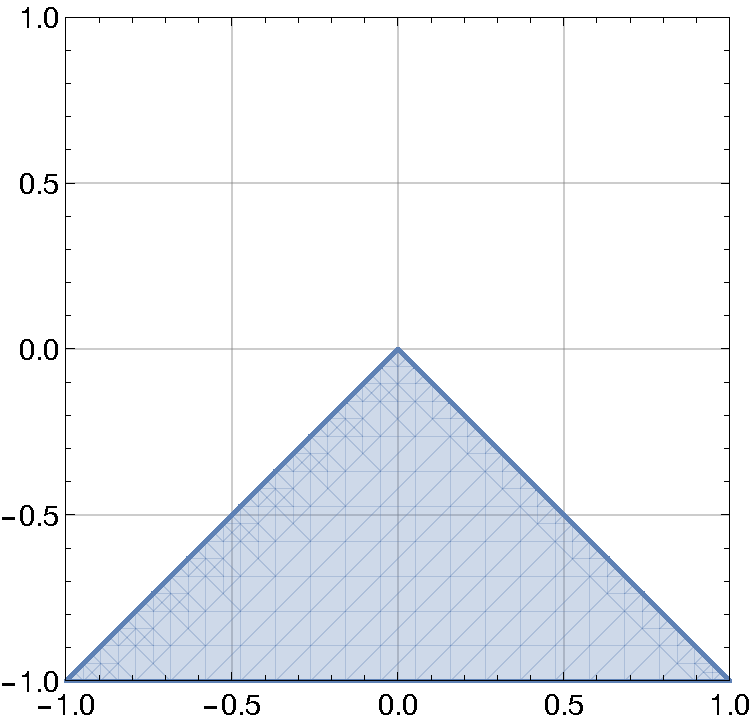
\includegraphics[width=1\linewidth]{plot_sampling01}
\end{minipage}
\quad
\begin{minipage}[b]{0.45\linewidth}
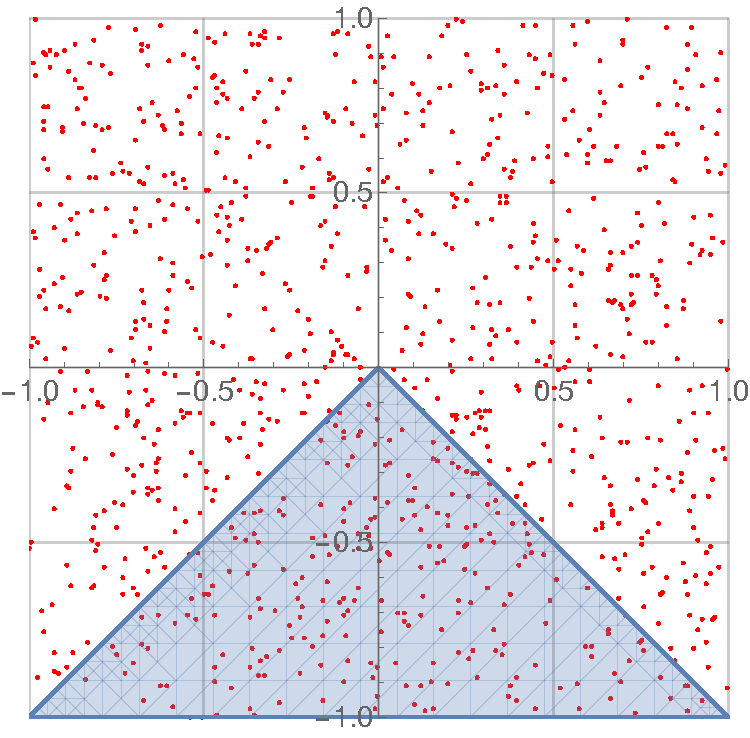
\includegraphics[width=1\linewidth]{plot_sampling02}
\end{minipage}
\caption{Sampling-based solution space quantification for $x \leq -y \land y \leq x$, $x, y \in [-1, 1]$.}
\label{fig:sampling-based}
\end{figure}

The hit-or-miss Monte Carlo method consists in taking $n$ independent random samples uniformly within the domain; if a sample $s_i$ satisfies the constraint, we assign $s_i=1$, otherwise, $s_i=0$. This process is called a Binomial experiment with $n$ samples. The maximum likelihood estimate for $p$ is then $\hat{p}$~\cite{pestman1998mathematical}:
%
\begin{equation}\label{eq:mleEstimator}
	\hat{p} = \frac{\sum_{i=1}^n s_i}{n} \qquad\qquad\qquad \sigma(\hat{p}) = \sqrt{\frac{\hat{p} \cdot (1-\hat{p})}{n}}
\end{equation}
%
The right part of Equation~\eqref{eq:mleEstimator} shows the standard deviation $\sigma$ of $\hat{p}$~\cite{pestman1998mathematical}. The standard deviation is an index of the convergence of the estimate. Notably, it decreases with the square root of the number of samples; when the number of samples grows to infinity, the standard deviation goes to $0$, making the estimation converge to the actual value of $p$.

Despite the convergence of $\hat{p}$ to $p$ can be proved only in the limit, given the value of $\hat{p}$, its standard deviation $\sigma$, and a desired confidence level $0<\alpha<1$, it is possible to define a confidence interval for the unknown value $p$. In particular:
%
\begin{equation}\label{eq:mleInterval}
	Pr\Big( \hat{p} - z_{\frac{\alpha}{2}} \cdot \sqrt{\frac{\hat{p} \cdot (1-\hat{p})}{n}} \ \leq p \leq \ \hat{p} + z_{\frac{\alpha}{2}} \cdot \sqrt{\frac{\hat{p} \cdot (1-\hat{p})}{n}} \Big) = 1-\frac{\alpha}{2}
\end{equation}
%
\noindent where $z_{\frac{\alpha}{2}}$ is the $1-\frac{\alpha}{2}$ quantile of the standard Gaussian distribution~\cite{pestman1998mathematical}.

Equation~\eqref{eq:mleInterval} is constructed using the central limit theorem, under the assumption that a large number of samples $n$ have been collected (as a rule of thumb, hundreds of samples or more are almost surely a good fit for this assumption). The width of the interval, which is an index of the accuracy of the estimate, can be arbitrarily reduced by increasing the number of samples $n$; thus, Equation~\eqref{eq:mleInterval} can be used as stopping criteria for the estimation process.

In our example, in a run with $n=10000$ samples, we obtained $\hat{p}= 0.2512$ with standard deviation $\sigma(\hat{p})=0.00433703$; thus, with $99\%$ confidence, we can conclude $p \in [0.248126, 0.254274]$. From Figure~\ref{fig:sampling-based}, it is easy to see that $p=0.25$, which falls within the computed interval.

Note that hit-or-miss methods may require a large number of samples to converge to a high accuracy (small interval). This is even worse when the actual value of $p$ is close to its extremes (0 or 1). Improvements on the convergence rates can be achieved using more complex sampling procedures such as quasi-Monte Carlo sampling~\cite{robert2013monte}, or importance sampling, Markov Chain Monte Carlo, or slice sampling~\cite{bishop2006pattern}; some of these methods have been used in probabilistic model checking~\cite{importanceSamplingSMC,splittingSMC,statisticalModelChecking}. 

Further more accurate confidence intervals can also be used as stopping criteria~\cite{pestman1998mathematical}; in probabilistic model checking, the most commonly used is the Chernoff-Hoeffding's bound~\cite{hoeffding1963probability,approximatePMC,statisticalModelChecking}. Bayesian estimators can also be used, allowing for the inclusion of prior knowledge on the expected result (when available)~\cite{Robert2007BayesianChoice,gelman2003bayesian}; the use of Bayesian methods led to faster convergence rate in many probabilistic verification problems~\cite{Zuliani:2010:BSM:1755952.1755987}. Finally, a hybrid approach, that  exploits interval constraint propagation and compositional solving has been proposed for probabilistic program analysis in~\cite{Borges2014,2015-fse-qcoral}.

\paragraph{Distribution-aware sampling.} The hit-or-miss Monte Carlo method we described offers a straightforward way to handle input distributions: the samples for the Binomial experiment can be simply drawn from the known distribution.
Efficient sampling algorithms exist for the most common continuous and discrete distributions, with off-the-shelf implementations for several programming languages (e.g.,~\cite{commonsMath3} for Java). A comprehensive survey of random number generation is beyond the scope of this paper (see e.g.~\cite{gentle2013random}). 
We describe here one of the simplest and most general techniques for this task: \emph{inverse CDF sampling}.


Assume our goal is to take a sample from a distribution $D$, e.g., a Gaussian distribution describing the inputs received by a temperature sensor. This distribution has a cumulative distribution function $CDF_D(x)$ representing the probability of observing a value less than or equal than $x$~\cite{pestman1998mathematical}. The value of the CDF is bounded between 0 and 1, for $x\to -\infty$ and $x \to \infty$, respectively. Furthermore, assuming every possible outcome has a strictly positive probability, as it is the case for most distributions used in practice, the CDF is strictly monotonic and invertible; let us denote its inverse $CDF_D^{-1}(\cdot)$. 

Inverse CDF sampling reduces sampling from $D$ to sampling from a Uniform distribution via the following three steps:

\begin{enumerate}
	\item generate a random sample $u$ from the Uniform distribution on $[0,1]$
	\item find the value $x$ such that $CDF_D(x)=u$, i.e., $CDF_D^{-1}(u)$
	\item return $x$ as the sample from $D$
\end{enumerate}

For example, to generate a sample from a Gaussian distribution $\mathcal{N}(10, 3)$, we first generate a sample $u$ from the uniform distribution in $[0,1]$, let's say 0.83; then, we compute $CDF^-1_{\mathcal{N}(10,3)}(0.83)=12.8625$, which is our sample input.

The computation of the CDF and its inverse is efficient for most univariate distributions used in practice, and implementations are available for all common programming languages. Multivariate distributions are usually more challenging, with only a few cases allowing direct solutions. Nonetheless, more complex computation methods exist (e.g., Gibbs sampling~\cite{Robert2005MCBook}), covering most of the practically useful distributions. Multivariate distributions are indeed useful to capture statistical dependence among input variables, whether this is know in the application domain or inferred from the data. Finally, the discretization method described in Section~\ref{sec:computingprobabilitiesExact} remains a viable general, approximate solution; however, distribution-aware sampling scales significantly better, especially when high accuracy is required~\cite{2015-fse-qcoral}.



\paragraph{Beyond numerical domains.}
Sampling-based methods are theoretically applicable for any input domain, provided a procedure for generating unbiased samples (according to the input distribution) is available. Solutions have been proposed for model counting of SAT problems (e.g., in~\cite{satCounting01,biere2009handbook,journalscorrMeel14}, also with distribution-aware approaches~\cite{chakraborty2014distribution}) and SMT problems (e.g., in~\cite{countingSMT}), while stochastic grammars can be used to generate random strings according to specified distributions~\cite{stochasticGrammars}. 
%
%
%Sampling-based probability computation described in this section is theoretically applicable to domains other than purely numeric ones. However, its practical implementation requires the ability to generate random inputs from these domains, possibly according to the input distributions specified by the developers. Random test case generation has developed effective techniques to generate random inputs for realistic programs. However, most of the techniques developed in this area do not provide any guarantee on the distribution of the generated inputs, possibly biasing the estimation process. 
%
%Sampling-based methods have been proposed for model counting of SAT problems (e.g., in~\cite{satCounting01,biere2009handbook,journalscorrMeel14}, also with distribution-aware approaches~\cite{chakraborty2014distribution}) and SMT problems (e.g., in~\cite{countingSMT}), while stochastic grammars can be used to generate random strings according to specified distributions~\cite{stochasticGrammars}.



%	\begin{itemize}
%		\item Sampling from uniform distributions (base case, best we can if no input distribution is available; based on classic probability, i.e., count success over total)
%		\item Discretization of non-uniform distributions (useful when a finite number of usage scenarios are available; can approximate any distribution with arbitrary accuracy; most straightforward when inferring distributions from past executions, i.e., histograms; it does not scale for fine-grained approximations)
%		\item Distribution-aware sampling (quite straightforward for distributions over numerical domains; requires more complex, unbiased, input generation techniques when sampling from other domains, e.g., data structures, but similar to random testing; scalability issues when sampling correlated input variables)
%      
%		\item Monte Carlo methods
%			\begin{itemize}
%				\item Hit or miss Monte Carlo
%				%\item \mycomment{Anto: Mention Crude montecarlo for integration? Gibbs and MCMC sampling will be just mentioned; especially MCMC is used by the MSR guys}
%				\item Frequentist and Bayesian estimators (used in prob. model check.)
%					\begin{itemize}
%						\item historically frequentist first, with static bounds (based on Chernoff's) for prob MC; then sequential ratio tests, still frequentist.
%						\item Bayesian from CMU
%					\end{itemize}
%				\item The variance issue and convergence acceleration techniques (just a paragraph with some refs):
%					\begin{itemize}
%						\item Importance sampling (used in prob. model check.)
%						\item Importance slicing (used in prob. model check.)
%					\end{itemize}
%
%				\item Exploiting he law of total probability for composing different estimators: Interval constraints propagation (PLDI14) and statistical/exact (FSE14)
%				\item Dealing with nondeterminism (freq and bayesian in prob MC, ASE14)	
%			\end{itemize}
%			
%			\item approximate $\sharp$-sat and $\sharp$-smt (\url{http://arxiv.org/pdf/1306.5726v3.pdf}, )
%	\end{itemize}


\ignore{
\subsection{Optimizations for PPA}\label{sec:computingprobabilitiesOptimizations}

While model counting and solution space quantification are general problems, their application to probabilistic program analysis can often be improved exploiting the additional information specific to this application field.

We briefly report in this section two techniques able to 1) exploit variables dependency to reduce the complexity of model counting and solution space quantification and 2) combine interval constraint propagation and stratified sampling to increase the accuracy of sampling-based probability computation, and in turn its convergence rate.

\paragraph{Divide and conquer.}
The complexity of all the model counting and solution space quantification techniques proposed in this section depends on the number of variables involved in the constraints to be quantified. Let us assume such constraints are provided in disjunctive normal form and that there is no intersection between the solution spaces of any pair of disjuncts (this is form is quite natural for most constraints analyzed in PPA, usually requiring low computational overhead for normalization). Since there is no intersection between the disjuncts, the solution space for each of them can be quantified separately and than summed up to obtain the result for the whole disjunction.

Let us focus on a single disjunct $\phi \equiv \phi_1 \land \phi_2 \land \dots \land \phi_n$ predicating on the variables $\{v_1, v_2, \dots, v_m\}$, i.e., for each $v_i$ there exists at least one conjunct $\phi_j$ predicating on its value. Our goal is to divide the quantification of the solution space of $\phi$ in a set of independent problems involving only a subset of the variables appearing in $\phi$. 

The central idea is that constraints in $\phi$ identify a dependency relation ($\textit{dep}$) among the constrained variables that can be formalized as follows (let $v_i$, $v_j$, and $v_k$ be variables in $\phi$ and $\phi_i$ be a conjunct in $\phi$):
\begin{itemize}
	\item $\forall v_i \ \textit{dep}(v_i,v_i)$
	\item $\forall v_i,v_j$ if there exist a conjunct $\phi_i$ predicating on both $v_i$ and $v_j$, then $\textit{dep}(v_i,v_j)$
	\item $\forall v_i,v_j,v_k$ $\textit{dep}(v_i,v_j) \land \textit{dep}(v_j,v_k) \implies \textit{dep}(v_i,v_k)$
\end{itemize}

The intuitive meaning of the $\textit{dep}$ relation is that if $\textit{dep}(v_i,v_j)$ then the values assumed by $v_i$ in a program run affect the values that can be assumed by $v_j$ towards the satisfaction of $\phi$. For example, from $\{x>5 \land y=x+5\}$ we deduce that the value of $y$ is affected by the values of $x$, and vice versa. The relation $\textit{dep}$ is an equivalence relation, thus it induces a partition on the set of variables appearing in $\phi$. For this reason, we can rewrite $\phi$ as the conjunction of the subsets $\phi_{[v]}$, each of whom collects all the constraints involving a variable in the equivalence class of $\textit{dep}$ represented by $v$. Such conjuncts are logically separated, hence it can be proved that $\textit{Pr}(\phi)= \prod_{v} \textit{Pr}(\phi_{[v]})$. 

For example, let $\phi$ be $\{x>2 \land y<5\}$, its probability can be computed as $\textit{Pr}(\phi)=\textit{Pr}(x>2) \cdot \textit{Pr}(y<5)$. The computation of the two probabilities on the right-hand side of this equality can be performed independently and each of them involves only one variable, reducing the effort of counting in a multidimensional space or taking samples from multidimensional distributions. Furthermore, the result of each subproblem can be cached and reused, with significant benefits in practical applications~\cite{Filieri2013}.


\paragraph{Interval constraint propagation and stratified sampling.}
Despite their generality, sampling-based methods for computing probability may suffer slow convergence rate. Several techniques have been established in statistics to mitigate this general issue~\cite{Robert2005MCBook}. Besides these techniques, the specificity of the problems we face in PPA can be exploited to define even more effective variance reduction technique.

Recall the example we introduced in Section~\ref{sec:computingprobabilitiesSampling}: we aim at quantifying the probability of satisfying the constraint 
$v_1 \leq -v_2 \land v_2 \leq v_1$, where both $v_1, v_2 \in [-1, 1] \cap \mathbb{R}$. Figure~\ref{fig:stratifiedICP} shows the domain and the solution space for this problem, with $v_1$ on the x-axis and $v_2$ on the y-axis. Using hit-or-miss Monte Carlo to solve this problem requires throwing random samples for $v_1$ and $v_2$ within their domain (i.e., from within the square), and computing the ratio between those falling within the shadowed triangle (i.e., satisfying the constraints) and the total number of samples. Geometrically, this corresponds to estimating the ratio between the area of the triangle and the area of the square (which is 1/4).

\begin{figure}[h!]\label{fig:stratifiedICP}
  \centering
      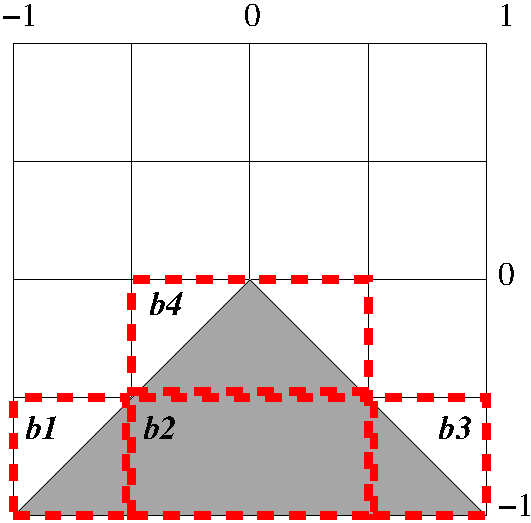
\includegraphics[width=3cm]{triangle}
  \caption{Example of ICP-based domain partitioning.}
\end{figure}

Looking at the figure it is evident that some regions of the domain do not contain solutions, i.e., the probability of satisfying the constraint within those regions is identically 0, without any estimation uncertainty. Intuitively, since we have an exact information about a fraction of the domain, we can confine the estimation, and consequently the uncertainty of estimation, only on the remaining part of the domain. This intuition can be systematized combining two techniques: interval constraint propagation and stratified sampling. 

Interval constraint propagation (ICP) is a algorithmic technique to compute interval solutions to equality and inequality numerical constraints. The input of ICP is a set of $n$ variables, each one defined on a convex domain, and a conjunction of numerical constraints; its output is a set of $n$-dimensional non-overlapping boxes whose union contains all the values of the variables satisfying all the constraints. Each box is essentially an hyperplane bounding a portion of the domain that contains solutions for the problem plus, possibly, other points that do not satisfy the constraint. Looking again at Figure~\ref{fig:stratifiedICP}, the application of ICP to our constraint produces the four 2-dimensional red boxes, whose union contains all the solutions. ICP can thus be used to partition the input domain into a set of regions, where each region may 1) contain no solutions, 2) contain only solutions, or 3) contain both solutions and values that do not satisfy the constraint. In the first two cases computing the probability will trivially lead to 0 and 1, respectively, without any uncertainty (i.e., zero variance). In the third case, sampling is needed to estimate the fraction of solution points.

When we have local results for each region in the domain partition, the second step is to compose these local information to obtain the probability estimate for the whole domain. Stratified sampling is a statistical techniques allowing to compose the local estimators of each region of the domain into a global estimator for the initial problem~\cite{Robert2005MCBook}. This computation is essentially a weighted sum of the local estimators, where the weight is the size of the region divided by the size of the domain. If we call $\hat{P}_i$ the local estimator of the $i$-th region and $w_i$ the ratio between the size of the $i$-th region and the size of the domain, exploiting the properties of expected value and variance for a sum of independent random variables~\cite{pestman1998mathematical}, we obtain for the global estimator $\hat{P}$ the following properties:

\begin{equation}\label{eq:stratifiedSampling}
	E[\hat{P}]=\sum_i w_i \cdot E[\hat{P}_i] \qquad Var[\hat{P}] = \sum_i w_i^2 \cdot Var[\hat{P}_i]
\end{equation}

The variance for the regions containing no solutions is trivially 0, thus the variance of the global estimator is reduced by the squared weight of these regions. Furthermore, for regions containing only solutions, the sampling-based probability computation will return variance 0 as well (recall Equation~\eqref{eq:mleEstimator}). Thus, fixed the total number of samples, the uncertainty on the global estimator with stratified sampling is always smaller or equal than the one we can obtain by applying Monte Carlo estimation on the whole domain, without partitions (this is a general result for stratified sampling~\cite{Robert2005MCBook}). 

The effectiveness of this approach depends on how much of the domain can be pruned out by the adopted ICP technique. This approach has been implemented in~\cite{Borges2014}, using the open-source ICP solver RealPaver~\cite{granvilliers2006tomas} for floating-point constraints, showing a significant reduction of the estimator variance on several realist programs, and, in turn, a faster convergence rate of the sampling-based probability computation. A combination of this technique with the previous divide and conquer strategy has been further developed in~\cite{2015-fse-qcoral} for a finer focusing of the sampling effort on the constraints and regions mostly affecting the variance of the global estimator, obtaining even faster convergence rates.






}






